\documentclass[conference,letterpaper]{IEEEtran}
\ifdefined\pdfminorversion\pdfminorversion=7\relax\fi
\usepackage[T1]{fontenc}
\usepackage[utf8]{inputenc}
\usepackage[english]{babel}
\usepackage{amsmath,amssymb}
\usepackage{graphicx,booktabs,array}
\usepackage{cite,url}
\usepackage{tikz}
\usetikzlibrary{arrows.meta,positioning}
\usepackage{float}
\usepackage[section]{placeins}
\usepackage{microtype}
\usepackage[hidelinks]{hyperref}

% The folder fig must be beside this .tex file.
\graphicspath{{fig/}}
\newcommand{\Ohm}{\Omega}
\newcommand{\kohm}{\mathrm{k}\Omega}
\newcommand{\uF}{\mu\mathrm{F}}
\newcommand{\nF}{\mathrm{nF}}
\newcommand{\V}{\mathrm{V}}
\newcommand{\A}{\mathrm{A}}
\newcommand{\W}{\mathrm{W}}
\newcommand{\Hz}{\mathrm{Hz}}
\newcommand{\kHz}{\mathrm{kHz}}
\tikzset{
    blk/.style={draw,rectangle,align=center,
        font=\footnotesize,minimum height=10mm,
        text width=21mm,inner sep=3pt},
    arr/.style={-{Latex[length=1.7mm]},line width=.5pt},
    aux/.style={blk,dashed}
}
\setlength{\tabcolsep}{3.5pt}
\setlength{\intextsep}{8pt plus 2pt minus 2pt}
\renewcommand{\arraystretch}{1.12}

\title{Discrete Electronics Project: Class AB Audio Amplifier\\
Design and Simulation Report}
\author{
\IEEEauthorblockN{
María Fernanda Morales Calderón, Ian José Álvarez Arrieta,\\
Oscar Felipe Montejo Cordero, Bryan Alessandro Elizondo Fallas,\\
Andrés Obregón López}
\IEEEauthorblockA{
School of Electronics Engineering\\
Tecnológico de Costa Rica (TEC)\\
Analog One}
}

\raggedbottom
\begin{document}
\maketitle
\begin{abstract}
Analog One develops a discrete audio amplifier that combines
preamplification, voltage gain, and a Class AB power stage for an
$8\,\Ohm$ loudspeaker. The design targets $20\,\W$ of output power
and uses commercial component values. Calculated values and simulation
results are organized in tables to summarize bias, signal levels,
and heat dissipation. The power-stage test delivered $22.8\,\W$
at $10\,\kHz$. The report also identifies the interstage checks
needed to assess the complete amplifier.
\end{abstract}
\begin{IEEEkeywords}
Audio amplifier, Class AB, discrete circuits, MOSFET, simulation.
\end{IEEEkeywords}

\section{Project Description}
The amplifier prepares an incoming audio signal, increases its voltage,
and delivers current to a loudspeaker. A BJT preamplifier provides
initial signal conditioning, a MOSFET voltage amplifier establishes the
power-stage input level, and a complementary Class AB output stage
drives the load. The design considers signal transfer, stable bias,
and component heating. Each stage is evaluated separately before the
complete signal path is assessed. A common $\pm24\,\V$ supply
serves the system: the preamplifier uses the positive rail and ground,
while the voltage and power stages use both rails.

\section{Block Diagrams}
\subsection{Overall Amplifier}
The three stages divide signal conditioning, voltage gain, and
loudspeaker drive into distinct functions.
\begin{figure}[H]
\centering
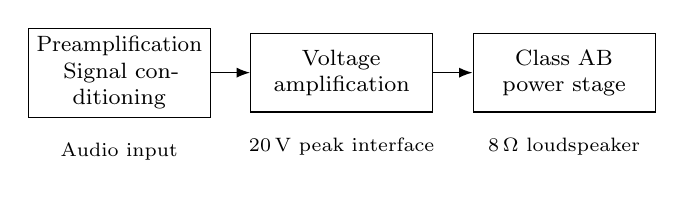
\begin{tikzpicture}[node distance=5mm]
\node[blk] (pre) {Preamplification\\Signal conditioning};
\node[blk,right=of pre] (gain) {Voltage\\amplification};
\node[blk,right=of gain] (power) {Class AB\\power stage};
\draw[arr] (pre)--(gain);
\draw[arr] (gain)--(power);
\node[below=2mm of pre,font=\scriptsize] {Audio input};
\node[below=2mm of gain,font=\scriptsize] {$20\,\V$ peak interface};
\node[below=2mm of power,font=\scriptsize] {$8\,\Ohm$ loudspeaker};
\end{tikzpicture}
\caption{Main stages of the audio amplifier.}
\label{fig:overall}
\end{figure}
\FloatBarrier
\subsection{Preamplification Stage}
The common-emitter stage increases the input signal level. Emitter
feedback helps stabilize its gain, while coupling capacitors keep the
DC bias separate from the adjacent stages.
\begin{figure}[H]
\centering
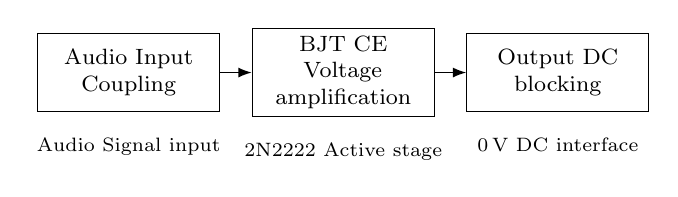
\begin{tikzpicture}[node distance=4mm]
\node[blk] (incoup) {Audio Input\\Coupling};
\node[blk,right=of incoup] (bjt) {BJT CE Voltage\\amplification};
\node[blk,right=of bjt] (outcoup) {Output DC\\blocking};
\draw[arr] (incoup)--(bjt);
\draw[arr] (bjt)--(outcoup);
\node[below=2mm of incoup,font=\scriptsize] {Audio Signal input};
\node[below=2mm of bjt,font=\scriptsize] {2N2222 Active stage};
\node[below=2mm of outcoup,font=\scriptsize] {$0\,\text{V}$ DC interface};
\end{tikzpicture}
\caption{Functional blocks of the BJT preamplifier stage.}
\label{fig:block_preamp}
\end{figure}
\FloatBarrier
\subsection{Voltage Amplification Stage}
Two common-source stages provide voltage gain while preserving the
signal polarity overall. An active load supplies current to the
second stage.
\begin{figure}[H]
\centering
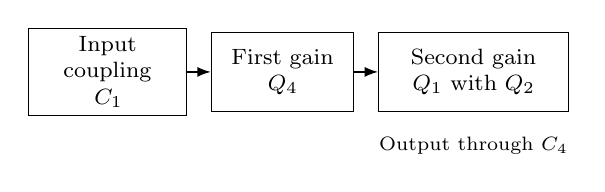
\begin{tikzpicture}[node distance=3mm]
\node[blk,text width=18mm] (a) {Input coupling\\$C_1$};
\node[blk,right=of a,text width=16mm] (b) {First gain\\$Q_4$};
\node[blk,right=of b,text width=22mm] (c) {Second gain\\$Q_1$ with $Q_2$};
\draw[arr] (a)--(b);
\draw[arr] (b)--(c);
\node[below=2mm of c,font=\scriptsize] {Output through $C_4$};
\end{tikzpicture}
\caption{Signal path through the voltage amplification stage.}
\label{fig:va_blocks}
\end{figure}
\FloatBarrier
\subsection{Class AB Power Stage}
Class AB operation was selected for its smooth transition between the
positive and negative portions of the signal and moderate resting
power consumption. The output stage supplies loudspeaker current
while retaining most of the input voltage amplitude
\cite[secs.~7--2 and 9--2]{floyd}.
\begin{figure}[H]
\centering
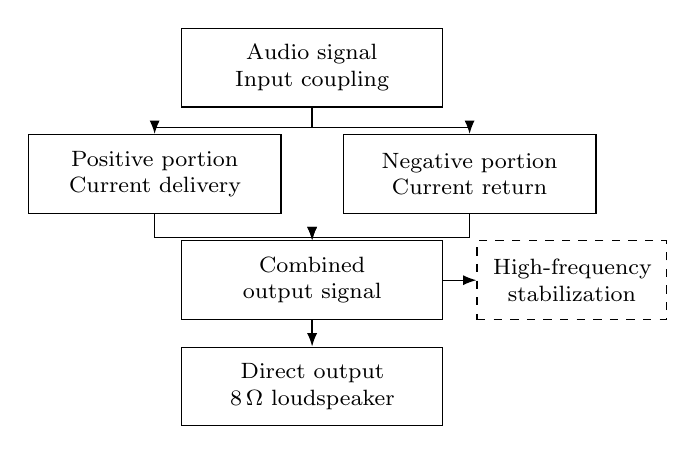
\begin{tikzpicture}
\node[blk,text width=31mm] (input) at (0,0)
    {Audio signal\\Input coupling};
\node[blk,text width=30mm] (n) at (-2,-1.35)
    {Positive portion\\Current delivery};
\node[blk,text width=30mm] (p) at (2,-1.35)
    {Negative portion\\Current return};
\node[blk,text width=31mm] (sum) at (0,-2.7)
    {Combined\\output signal};
\node[blk,text width=31mm] (speaker) at (0,-4.05)
    {Direct output\\$8\,\Ohm$ loudspeaker};
\node[aux,text width=22mm] (z) at (3.3,-2.7)
    {High-frequency\\stabilization};
\draw[arr] (input.south)--++(0,-.25)-|(n.north);
\draw[arr] (input.south)--++(0,-.25)-|(p.north);
\draw[arr] (n.south)--++(0,-.3)-|(sum.north);
\draw[arr] (p.south)--++(0,-.3)-|(sum.north);
\draw[arr] (sum)--(speaker);
\draw[arr] (sum)--(z);
\end{tikzpicture}
\caption{Functional blocks of the selected Class AB output arrangement.}
\label{fig:powerblock}
\end{figure}
\FloatBarrier

\section{Design Considerations and Calculated Values}
\subsection{Preamplification Stage}
The preamplifier uses a common-emitter 2N2222 with an unbypassed
emitter resistor. Its bias network uses the positive supply rail and
ground. Table~\ref{tab:preamp_calc} summarizes the nominal
operating point of this configuration.
\begin{figure}[H]
\centering
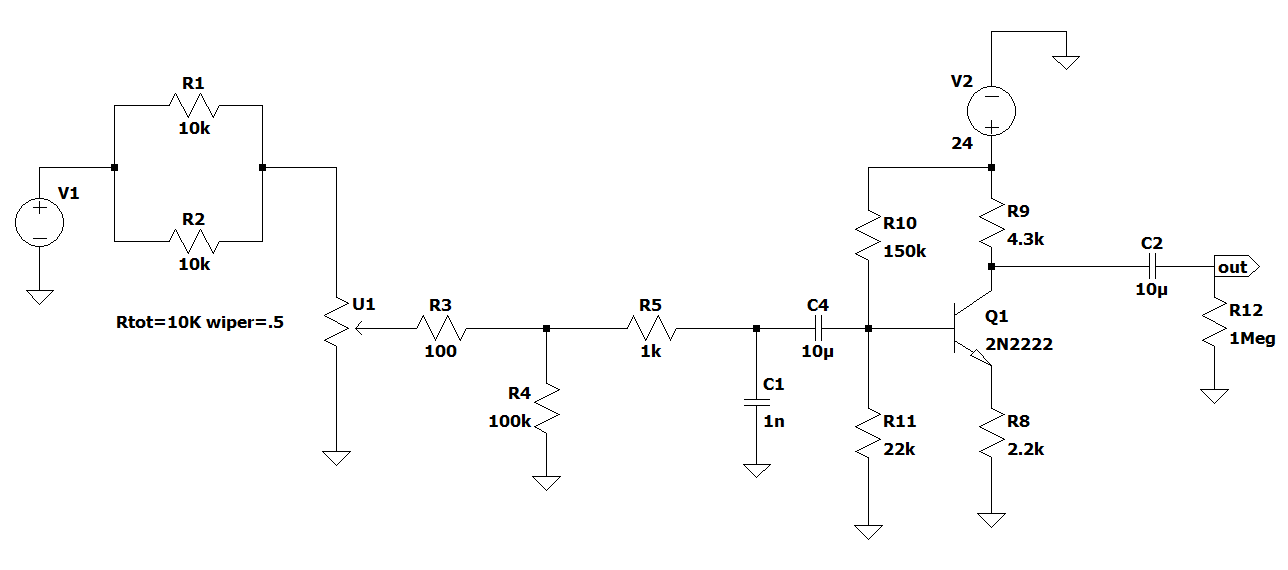
\includegraphics[width=\columnwidth]{pre_diam.png}
\caption{2N2222 preamplifier test circuit.}
\label{fig:pre_diam}
\end{figure}
\FloatBarrier
\begin{table}[H]
\caption{Calculated Preamplifier Design Values}
\label{tab:preamp_calc}
\centering\footnotesize
\setlength{\tabcolsep}{2pt}
\begin{tabular}{@{}p{0.62\columnwidth}p{0.33\columnwidth}@{}}
\toprule
Quantity & Value\\
\midrule
Base-network equivalent resistance & $19.19\,\kohm$\\
Base-network open-circuit voltage & $3.07\,\V$\\
Base current & $6.744\,\mu\A$\\
Base voltage & $2.94\,\V$\\
Emitter voltage & $2.24\,\V$\\
Collector voltage & $19.65\,\V$\\
Collector current & $1.012\,\mathrm{mA}$\\
Emitter current & $1.018\,\mathrm{mA}$\\
Collector-to-emitter voltage & $17.41\,\V$\\
Dynamic emitter resistance & $25.55\,\Ohm$\\
Nominal unloaded voltage gain & $-1.93\,\mathrm{V/V}$\\
Transistor resting loss & $17.61\,\mathrm{mW}$\\
Estimated junction temperature & $28.52\,{}^\circ\mathrm{C}$\\
\bottomrule
\end{tabular}
\par\smallskip
\parbox{.97\columnwidth}{\scriptsize Nominal calculation uses the $+24\,\V$ rail, ground, a current-gain parameter of 150, a base-to-emitter drop of $0.70\,\V$, and $25\,{}^\circ\mathrm{C}$ ambient.}
\end{table}
\FloatBarrier
\subsection{Voltage Amplification Stage}
The voltage stage establishes the signal level required by the power
stage. Table~\ref{tab:va_calc} summarizes its calculated interface
values. Bias estimates include the recorded resting drain voltages.
\begin{figure}[H]
\centering
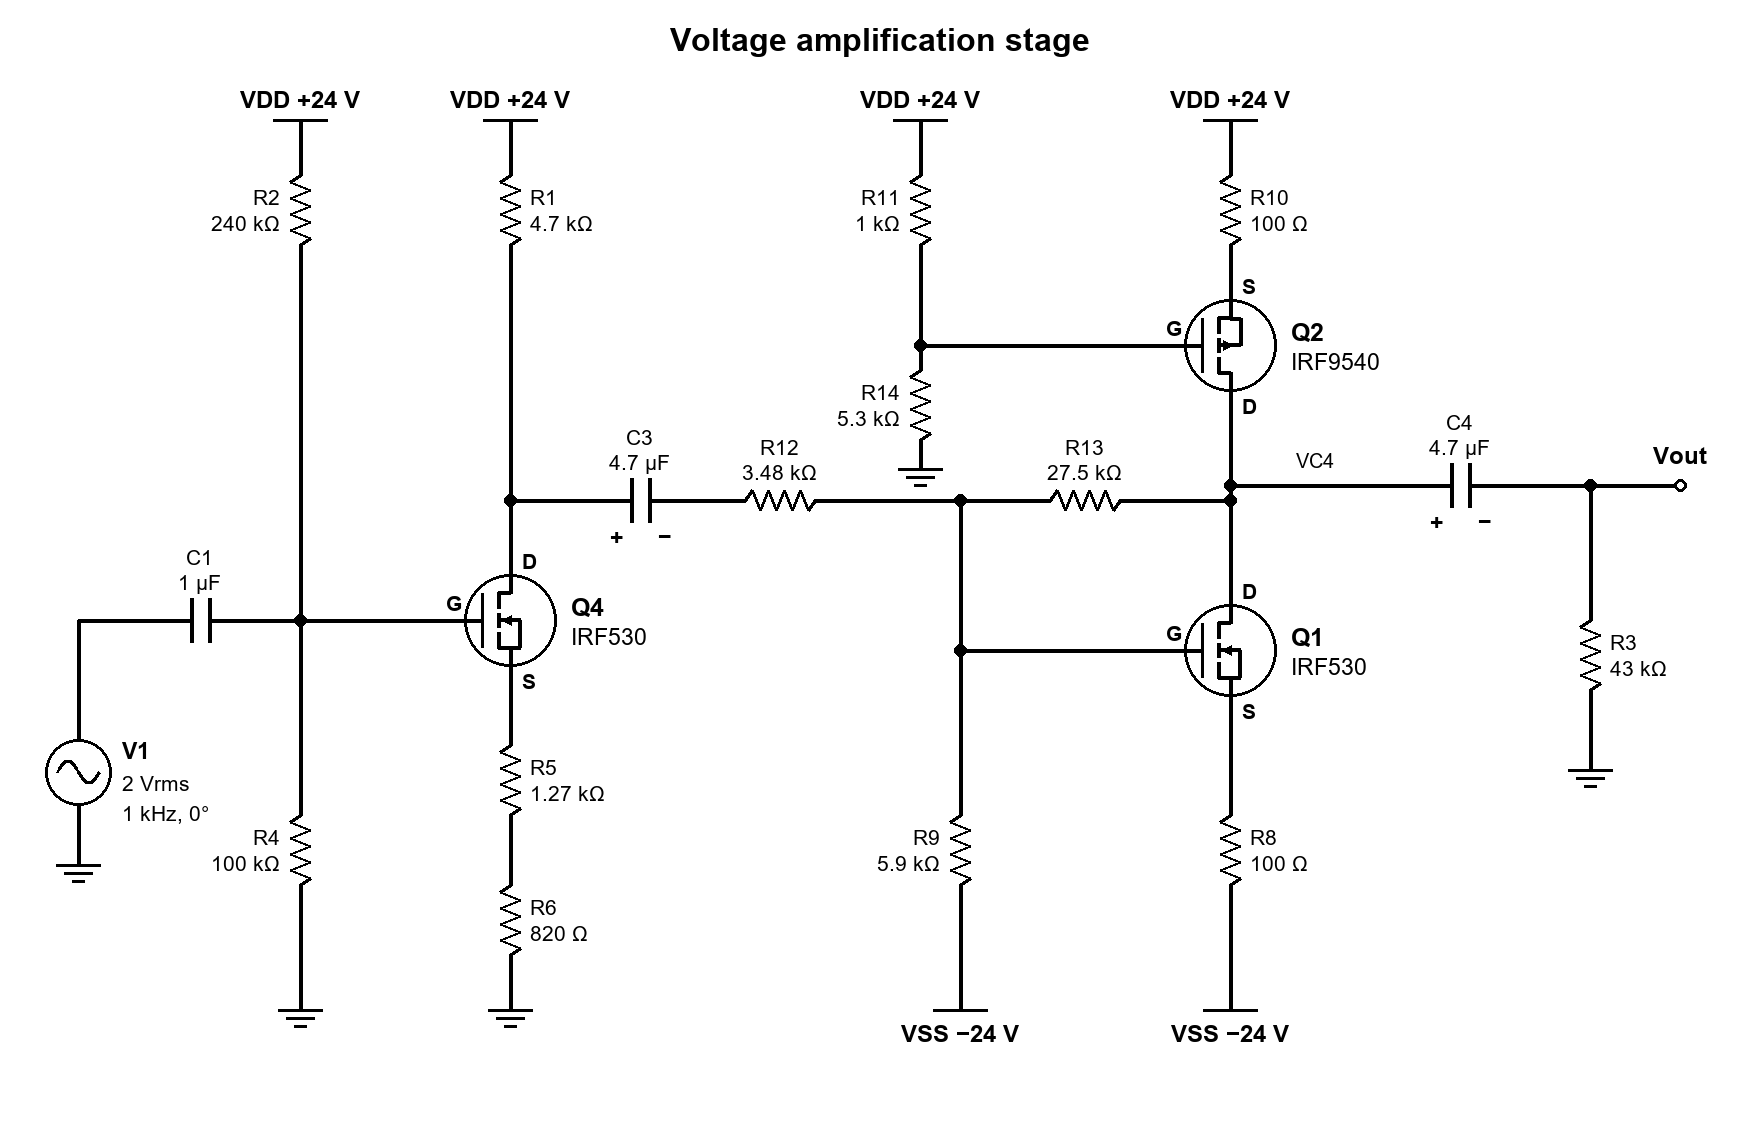
\includegraphics[width=\columnwidth]{AS.png}
\caption{MOSFET voltage amplifier with an active load and a
$43\,\kohm$ test load.}
\label{fig:va_schematic}
\end{figure}
\FloatBarrier
\begin{table}[H]
\caption{Calculated Voltage-Stage Interface Values}
\label{tab:va_calc}
\centering\footnotesize
\setlength{\tabcolsep}{2pt}
\begin{tabular}{@{}p{0.62\columnwidth}p{0.33\columnwidth}@{}}
\toprule
Quantity & Value\\
\midrule
Required output, peak & $20.00\,\V$\\
Required output, RMS & $14.14\,\V$\\
Required voltage gain & $7.07\,\mathrm{V/V}$\\
Input resistance & $70.6\,\kohm$\\
Input coupling corner & $2.25\,\Hz$\\
Load current at target, RMS & $0.329\,\mathrm{mA}$\\
Load power at target & $4.65\,\mathrm{mW}$\\
First-stage source resistance & $2.09\,\kohm$\\
DC feedback-path current & $0.715\,\mathrm{mA}$\\
Active-load bias-divider current & $3.81\,\mathrm{mA}$\\
R11 resting loss & $14.5\,\mathrm{mW}$\\
R14 resting loss & $76.9\,\mathrm{mW}$\\
Q4 gate-to-source voltage & $3.90\,\V$\\
Q4 drain-to-source voltage & $13.73\,\V$\\
\bottomrule
\end{tabular}
\end{table}
\FloatBarrier
\begin{table}[H]
\caption{Calculated Voltage-Stage Bias and Resting Losses}
\label{tab:va_bias}
\centering\footnotesize
\setlength{\tabcolsep}{2pt}
\begin{tabular}{@{}p{0.11\columnwidth}p{0.2\columnwidth}p{0.2\columnwidth}p{0.19\columnwidth}p{0.21\columnwidth}@{}}
\toprule
Device & Gate (V) & Source (V) & Current (mA) & Loss (mW)\\
\midrule
Q4 & $7.06$ & $3.16$ & $1.51$ & $20.8$\\
Q1 & $-19.78$ & $-23.69$ & $3.07$ & $72$\\
Q2 & $20.19$ & $23.62$ & $3.79$ & $90$\\
\bottomrule
\end{tabular}
\par\smallskip
\parbox{.97\columnwidth}{\scriptsize Q1 and Q2 entries are nominal resting estimates.}
\end{table}
\FloatBarrier
\subsection{Class AB Power Stage}
The complementary source followers supply current directly to the
loudspeaker. Adjustable gate bias sets a small resting drain current
and keeps the output near zero DC.
\begin{figure}[H]
\centering
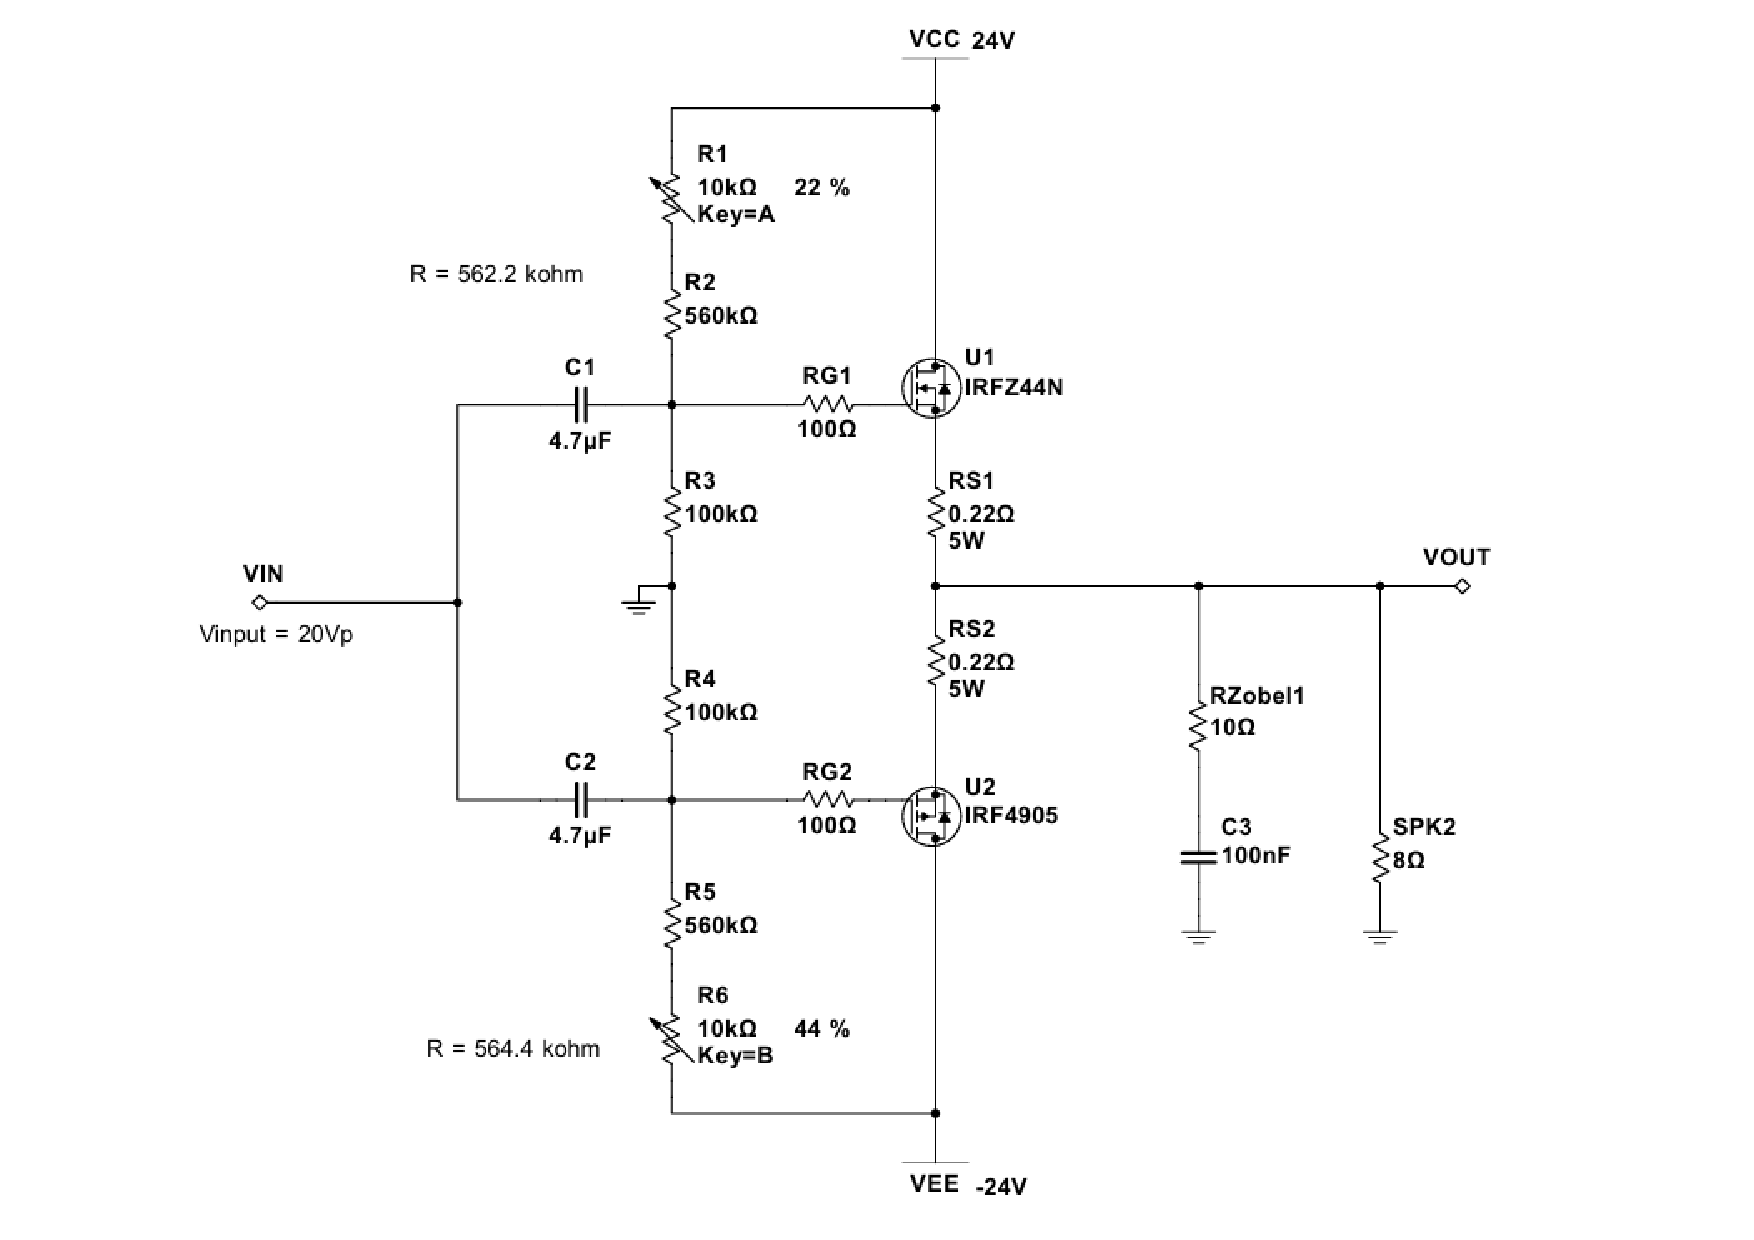
\includegraphics[width=\columnwidth,
    trim=84.5bp 11bp 115.5bp 3bp,clip]{pot20w(3).pdf}
\caption{Class AB power-stage schematic with IRFZ44N and IRF4905
MOSFETs.}
\label{fig:schematic}
\end{figure}
\FloatBarrier
\begin{table}[H]
\caption{Calculated Power-Stage Design Values}
\label{tab:power_calc}
\centering\footnotesize
\setlength{\tabcolsep}{2pt}
\begin{tabular}{@{}p{0.62\columnwidth}p{0.33\columnwidth}@{}}
\toprule
Quantity & Value\\
\midrule
Output-power target & $20\,\W$\\
Required load voltage, RMS & $12.65\,\V$\\
Required load voltage, peak & $17.89\,\V$\\
Required load voltage, peak-to-peak & $35.78\,\V$\\
Required load current, RMS & $1.58\,\A$\\
Required load current, peak & $2.24\,\A$\\
Upper gate bias, initial & $+3.6243\,\V$\\
Lower gate bias, initial & $-3.6123\,\V$\\
Upper effective bias resistance & $562.2\,\kohm$\\
Lower effective bias resistance & $564.4\,\kohm$\\
R1 effective setting & $2.2\,\kohm$ ($22\%$)\\
R6 effective setting & $4.4\,\kohm$ ($44\%$)\\
Quiescent drain current, $I_{DQ}$ & $50\,\mathrm{mA}$ per device\\
Resting drop across RS1 and RS2 & $11\,\mathrm{mV}$ each\\
Output DC target & $0\,\V$\\
Input resistance per branch & $84.9\,\kohm$\\
Input coupling corner & $0.40\,\Hz$\\
Resting loss per source resistor & $0.55\,\mathrm{mW}$\\
\bottomrule
\end{tabular}
\par\smallskip
\parbox{.97\columnwidth}{\scriptsize The initial gate settings are adjusted through the zero-input DC analysis to meet the resting-current and output-DC targets.}
\end{table}
\FloatBarrier
\subsubsection{Heat Dissipation}
The thermal assessment uses an ambient temperature of
$25\,{}^\circ\mathrm{C}$ for all components. Each output transistor
uses a separate NTE495 aluminum heat sink for natural-convection
cooling \cite{nte495}.
\begin{table}[H]
\caption{Power-Stage Losses and Calculated Temperatures}
\label{tab:thermal}
\centering\footnotesize
\setlength{\tabcolsep}{2pt}
\begin{tabular}{@{}p{0.25\columnwidth}p{0.36\columnwidth}p{0.32\columnwidth}@{}}
\toprule
Component & Power used & Temperature (${}^\circ\mathrm{C}$)\\
\midrule
U1 & $6.58\,\W$ & $123.7$\\
U2 & $6.63\,\W$ & $119.5$\\
R1 & $4.28\,\mu\W$ & $25.0$\\
R2 & $1.09\,\mathrm{mW}$ & $25.2$\\
R3, R4 & $2.13\,\mathrm{mW}$ & $25.3$\\
R5 & $1.08\,\mathrm{mW}$ & $25.2$\\
R6 & $8.50\,\mu\W$ & $25.0$\\
RG1 & $0.171\,\mathrm{mW}$ & $25.0$\\
RG2 & $0.913\,\mathrm{mW}$ & $25.1$\\
RS1, RS2 & $0.732\,\W$ & $65.3$\\
RZobel1 & $0.0714\,\W$ & $30.4$\\
C1 & $0.0590\,\mathrm{mW}$ & $25.0$\\
C2 & $0.311\,\mathrm{mW}$ & $25.1$\\
C3 & $0.0284\,\W$ & $57.9$\\
\bottomrule
\end{tabular}
\par\smallskip
\parbox{.97\columnwidth}{\scriptsize Temperatures are analytical estimates. U1/U2 entries refer to the junction; passive entries refer to the body. Grouped values apply to each component. RS1/RS2 use a sizing allowance; U1/U2 powers are recorded test losses.}
\end{table}
\FloatBarrier
\begin{table}[H]
\caption{Calculated Output-Transistor Thermal Conditions}
\label{tab:thermal_conditions}
\centering\footnotesize
\setlength{\tabcolsep}{2pt}
\begin{tabular}{@{}p{0.33\columnwidth}p{0.23\columnwidth}p{0.18\columnwidth}p{0.18\columnwidth}@{}}
\toprule
Condition & Loss per device & U1 (${}^\circ\mathrm{C}$) & U2 (${}^\circ\mathrm{C}$)\\
\midrule
Resting target & $1.20\,\W$ & $43.0$ & $42.1$\\
Thermal stress check & $10\,\W$ & $175.0$ & $167.5$\\
\bottomrule
\end{tabular}
\par\smallskip
\parbox{.97\columnwidth}{\scriptsize Estimates use a constant-resistance model: one NTE495 per device at $13\,{}^\circ\mathrm{C/W}$ and a $0.5\,{}^\circ\mathrm{C/W}$ mounting interface. The heat-sink rating is specified at a $75\,{}^\circ\mathrm{C}$ rise in natural convection \cite{nte495}. Both MOSFETs have a maximum junction temperature of $175\,{}^\circ\mathrm{C}$ \cite{irfz44n,irf4905}; the $10\,\W$ check leaves no thermal margin for U1.}
\end{table}
\FloatBarrier

\section{Component Selection Criteria}
\subsection{Preamplification Stage}
The bias divider sets the transistor operating point, while the
emitter resistor provides local feedback. Coupling capacitors isolate
the DC levels of adjacent stages.
\begin{table}[H]
\caption{Preamplifier Components}
\label{tab:preamp_components}
\centering\footnotesize
\setlength{\tabcolsep}{2pt}
\begin{tabular}{@{}p{.20\columnwidth}p{.29\columnwidth}p{.44\columnwidth}@{}}
\toprule
Reference & Value & Function\\
\midrule
Q1 & 2N2222 & Common-emitter amplifier\\
R10 & $150\,\kohm$ & Upper bias resistor\\
R11 & $22\,\kohm$ & Lower bias resistor\\
R9 & $4.3\,\kohm$ & Collector resistor\\
R8 & $2.2\,\kohm$ & Emitter feedback\\
C4, C2 & $10\,\uF$ each & Input and output coupling\\
R12 & $1\,\mathrm{M}\Ohm$ & Output return\\
C1 & $1\,\nF$ & High-frequency filtering\\
R3 & $100\,\Ohm$ & Input series resistor\\
R4 & $100\,\kohm$ & Input return\\
R5 & $1\,\kohm$ & Filter resistor\\
U1 & $10\,\kohm$ & Input volume control\\
\bottomrule
\end{tabular}
\end{table}
\FloatBarrier
\subsection{Voltage Amplification Stage}
IRF530 devices provide voltage gain, while an IRF9540 acts as the
active load \cite{va_irf530,va_irf9540}. The input and feedback
resistances set the gain and loading between the stages.
\begin{table}[H]
\centering\footnotesize
\caption{Voltage-Stage Components}
\label{tab:va_parts}
\begin{tabular}{@{}p{.21\columnwidth}p{.33\columnwidth}p{.39\columnwidth}@{}}
\toprule
Reference & Value & Function\\
\midrule
$Q_4$, $Q_1$ & IRF530 & Common-source gain\\
$Q_2$ & IRF9540 & Active load\\
$R_2$, $R_4$ & $240\,\kohm$, $100\,\kohm$ & $Q_4$ gate bias\\
$R_1$ & $4.7\,\kohm$ & $Q_4$ drain load\\
$R_5$, $R_6$ & $1.27\,\kohm$, $820\,\Ohm$ & $Q_4$ source path\\
$R_{12}$, $R_{13}$ & $3.48\,\kohm$, $27.5\,\kohm$ & Input and feedback\\
$R_9$ & $5.9\,\kohm$ & Return to $-24\,\V$\\
$R_8$, $R_{10}$ & $100\,\Ohm$ each & Source resistors\\
$R_{11}$, $R_{14}$ & $1\,\kohm$, $5.3\,\kohm$ & $Q_2$ gate bias\\
$R_3$ & $43\,\kohm$ & Output test load\\
$C_1$ & $1\,\uF$ & Nonpolar input coupling\\
$C_3$, $C_4$ & $4.7\,\uF$ each & Interstage and output\\
\bottomrule
\end{tabular}
\end{table}
\FloatBarrier
\subsection{Class AB Power Stage}
The complementary MOSFETs share the load current. Source resistors
provide bias-current checks, and the output RC network supports
high-frequency operation \cite{irfz44n,irf4905}.
\begin{table}[H]
\caption{Power-Stage Components and Selection Ratings}
\label{tab:components}
\centering\footnotesize
\begin{tabular}{@{}p{.18\columnwidth}p{.30\columnwidth}p{.46\columnwidth}@{}}
\toprule
Reference & Value or model & Selection rating\\
\midrule
U1 & IRFZ44N & N-channel MOSFET\\
U2 & IRF4905 & P-channel MOSFET\\
R2, R5 & $560\,\kohm$ & $1\%$, $0.25\,\W$\\
R3, R4 & $100\,\kohm$ & $1\%$, $0.25\,\W$\\
R1, R6 & $10\,\kohm$ & Trimmers, $0.25\,\W$\\
RG1, RG2 & $100\,\Ohm$ & $0.25\,\W$\\
RS1, RS2 & $0.22\,\Ohm$ & $5\,\W$\\
C1, C2 & $4.7\,\uF$ & $50\,\V$, electrolytic\\
RZobel1 & $10\,\Ohm$ & $2\,\W$\\
C3 & $100\,\nF$ & $50\,\V$, ceramic, code 104\\
SPK2 & $8\,\Ohm$ & $30\,\W$ nominal rating\\
HS1, HS2 & NTE495 & Two heat sinks, one per MOSFET\\
\bottomrule
\end{tabular}
\end{table}
\FloatBarrier

\subsubsection{Heat-Sink Recommendations}
The NTE495 supplied by Teltron is selected for both output devices.
Table~\ref{tab:heatsink_options} also lists two compact local
alternatives. Their thermal resistance must be confirmed before
either replaces the selected model.
\begin{table}[H]
\caption{Compact Heat-Sink Options in Costa Rica}
\label{tab:heatsink_options}
\centering\footnotesize
\setlength{\tabcolsep}{2pt}
\begin{tabular}{@{}p{.34\columnwidth}p{.27\columnwidth}p{.32\columnwidth}@{}}
\toprule
Model and supplier & Size (mm) & Thermal information\\
\midrule
NTE495, Teltron & $29.9\times25.4\times12.7$ & $13\,{}^\circ\mathrm{C/W}$; selected \cite{nte495}\\
AD73819, MicroJPM & $43\times17\times30$ & Rating not published \cite{microjpm_heatsink}\\
DEV-CB0214-68, CRCibern\'etica & $50\times45\times18$ & Rating not published \cite{crc_heatsink}\\
\bottomrule
\end{tabular}
\par\smallskip
\parbox{.97\columnwidth}{\scriptsize NTE495 data follow the manufacturer's datasheet. Alternative dimensions follow supplier product specifications; manufacturer datasheets are not provided in those listings.}
\end{table}
\FloatBarrier

\section{Simulation Methodology}
DC analysis evaluates resting bias. Transient tests measure signal
levels and power, while frequency sweeps and harmonic analysis assess
signal transfer and distortion. LTspice and Multisim were used for the
preamplifier; the voltage and power stages were evaluated in Multisim.
\begin{table}[H]
\caption{Stage Test Conditions}
\label{tab:test_conditions}
\centering\footnotesize
\setlength{\tabcolsep}{2pt}
\begin{tabular}{@{}p{0.35\columnwidth}p{0.28\columnwidth}p{0.3\columnwidth}@{}}
\toprule
Stage & Signal & Load or condition\\
\midrule
Preamplifier & $1\,\kHz$ transient & DC and AC sweep\\
Voltage amplifier & $2\,\V$ RMS, $1\,\kHz$ & $43\,\kohm$\\
Power amplifier & $20\,\V$ peak, $10\,\kHz$ & $8\,\Ohm$\\
\bottomrule
\end{tabular}
\par\smallskip
\parbox{.97\columnwidth}{\scriptsize All tests use the common $\pm24\,\V$ supply; the preamplifier draws from $+24\,\V$ and ground. Voltage-stage Fourier analysis includes nine harmonics with a $2\,\mathrm{s}$ stop time to allow settling. Power-stage bias is checked with zero audio input.}
\end{table}
\FloatBarrier

\section{Simulated Values and Results}
\subsection{Preamplification Stage}
Table~\ref{tab:preamp_sim_dc} compares the nominal DC bias with
the recorded simulation for this configuration.
\begin{table}[H]
\caption{Preamplifier DC Bias Results}
\label{tab:preamp_sim_dc}
\centering\footnotesize
\setlength{\tabcolsep}{2pt}
\begin{tabular}{@{}p{0.38\columnwidth}p{0.2\columnwidth}p{0.2\columnwidth}p{0.16\columnwidth}@{}}
\toprule
Quantity & Calculated & Simulated & Deviation\\
\midrule
Base voltage & $2.94\,\V$ & $3.03\,\V$ & $3.06\%$\\
Emitter voltage & $2.24\,\V$ & $2.33\,\V$ & $4.02\%$\\
Collector voltage & $19.65\,\V$ & $19.47\,\V$ & $0.92\%$\\
Collector current & $1.012\,\mathrm{mA}$ & $1.055\,\mathrm{mA}$ & $4.25\%$\\
Collector-to-emitter voltage & $17.41\,\V$ & $17.14\,\V$ & $1.55\%$\\
Output DC & $0\,\V$ & $194.66\,\mathrm{pV}$ & ---\\
\bottomrule
\end{tabular}
\end{table}
\FloatBarrier
\begin{table}[H]
\caption{Reported Preamplifier Transient Output}
\label{tab:preamp_transient}
\centering\footnotesize
\setlength{\tabcolsep}{2pt}
\begin{tabular}{@{}p{0.62\columnwidth}p{0.33\columnwidth}@{}}
\toprule
Quantity & Value\\
\midrule
Output, peak-to-peak & Approximately $1.0\,\V$\\
Output, peak & Approximately $0.50\,\V$\\
Output DC center & $0\,\V$\\
\bottomrule
\end{tabular}
\end{table}
\FloatBarrier
\subsection{Voltage Amplification Stage}
The transient test reaches the required output swing. The Fourier
results summarize the fundamental and harmonic content after the
coupling capacitors have settled.
\begin{figure}[H]
\centering
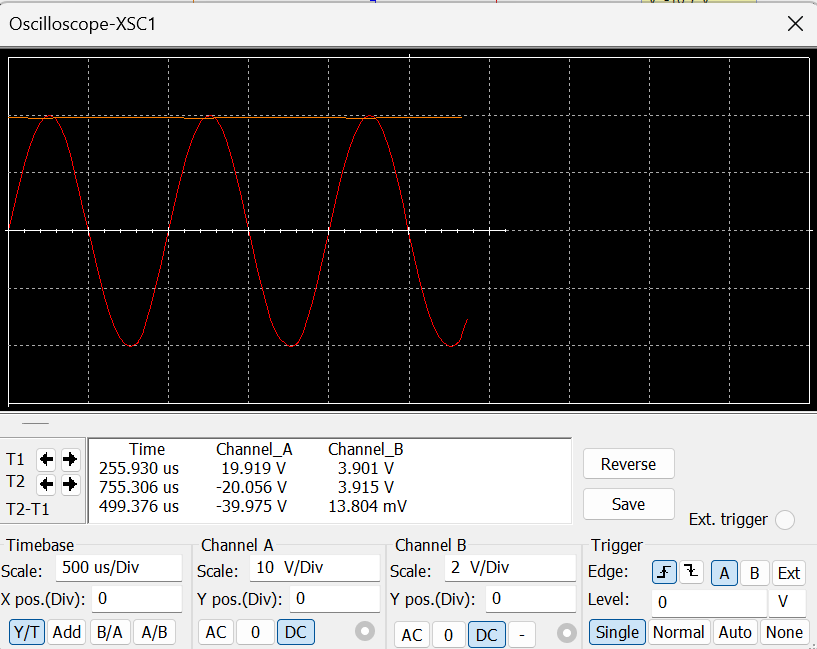
\includegraphics[width=\columnwidth]{fig/Voltage_Amplification_1kHz.png}
\caption{Voltage-stage transient test at $1\,\kHz$; cursors mark opposite output peaks.}
\label{fig:va_scope}
\end{figure}
\FloatBarrier
\begin{table}[H]
\caption{Voltage-Stage Simulation Results}
\label{tab:va_results}
\centering\footnotesize
\setlength{\tabcolsep}{2pt}
\begin{tabular}{@{}p{0.62\columnwidth}p{0.33\columnwidth}@{}}
\toprule
Quantity & Value\\
\midrule
Q4 drain at rest & $16.89\,\V$\\
Internal output at rest, VC4 & $-0.125\,\V$\\
Positive output peak & $19.919\,\V$\\
Negative output peak & $-20.056\,\V$\\
Output DC, Fourier analysis & $0.996\,\mathrm{mV}$\\
Fundamental amplitude & $20.112\,\V$ peak\\
Second harmonic & $0.077\,\V$ peak\\
Third harmonic & $0.193\,\V$ peak\\
THD, through ninth harmonic & $1.183\%$\\
Small-signal gain near $20\,\Hz$ & $6.930\,\mathrm{V/V}$\\
Small-signal gain near $1\,\kHz$ & $7.118\,\mathrm{V/V}$\\
Derived output swing & $39.975\,\V$ peak-to-peak\\
Derived transient gain & $7.07\,\mathrm{V/V}$\\
Fundamental, RMS equivalent & $14.22\,\V$\\
Output-swing target deviation & Less than $0.07\%$\\
\bottomrule
\end{tabular}
\end{table}
\FloatBarrier
\subsection{Class AB Power Stage}
The recorded test delivers more than the target load power.
The transistor losses represent heat in the output devices and are
separate from the power delivered to the loudspeaker.
\begin{table}[H]
\caption{Power-Stage Voltages at $10\,\kHz$}
\label{tab:voltages}
\centering\footnotesize
\setlength{\tabcolsep}{2pt}
\begin{tabular}{@{}p{0.36\columnwidth}p{0.18\columnwidth}p{0.18\columnwidth}p{0.22\columnwidth}@{}}
\toprule
Location & Peak-to-peak & RMS & DC mean\\
\midrule
IRFZ44N gate & $39.9\,\V$ & $14.6\,\V$ & $+3.62\,\V$\\
IRF4905 gate & $39.8\,\V$ & $14.6\,\V$ & $-3.62\,\V$\\
Output AC & $38.2\,\V$ & $13.5\,\V$ & ---\\
\bottomrule
\end{tabular}
\par\smallskip
\parbox{.97\columnwidth}{\scriptsize The output DC mean is not included in this test record. Its adjustment target appears in Table~\ref{tab:power_calc}.}
\end{table}
\FloatBarrier
\begin{table}[H]
\caption{Power-Stage Current and Power Results}
\label{tab:powers}
\centering\footnotesize
\setlength{\tabcolsep}{2pt}
\begin{tabular}{@{}p{0.62\columnwidth}p{0.33\columnwidth}@{}}
\toprule
Quantity & Value\\
\midrule
Load current, peak-to-peak & $4.78\,\A$\\
Load current, RMS & $1.69\,\A$\\
Average load power, simulated & $22.8\,\W$\\
U1 average loss, simulated & $6.58\,\W$\\
U2 average loss, simulated & $6.63\,\W$\\
Load power derived from RMS voltage & $22.78\,\W$\\
Load current derived from RMS voltage & $1.69\,\A$\\
Output peak derived from voltage swing & $19.1\,\V$\\
Output-to-input amplitude ratio & $95.5\%$\\
Power above design target & $14\%$\\
\bottomrule
\end{tabular}
\end{table}
\FloatBarrier

\section{Analysis and Integration}
\subsection{Preamplification Stage}
The calculated and simulated DC values place the transistor in its
active region. Coupling capacitors isolate this bias from the next
stage. The interstage check measures signal gain with the voltage
amplifier connected.

\subsection{Voltage Amplification Stage}
The final resistor network balances the required output swing and
harmonic distortion. Its standalone load test establishes the voltage
available to the next stage; the connected power-stage input adds
loading that must be included in the interface check.

\subsection{Class AB Power Stage}
The load-voltage and current readings support the recorded output
power. The amplitude ratio is consistent with a source follower,
and the recorded transistor losses define the heat-sink operating point.
The preceding stage must sustain the required voltage under the
connected input load.

\section{Conclusions and Next Steps}
\subsection{Preamplification Stage}
The BJT stage provides initial voltage gain and DC isolation using
the positive supply rail. Loaded interstage measurements complete
its integration into the signal path.

\subsection{Voltage Amplification Stage}
The MOSFET voltage stage reaches the required signal swing with
controlled harmonic distortion in the standalone test. The next
check is its output with the power-stage input connected.

\subsection{Class AB Power Stage}
The complementary output stage meets the power objective in the
recorded test. Its thermal assessment uses one NTE495 heat sink per
output transistor at the recorded losses. Loaded interstage measurements,
frequency response, and signal-quality checks complete the amplifier
assessment.
\begin{thebibliography}{8}
\bibitem{floyd}
T. L. Floyd, \emph{Dispositivos electrónicos}, 8th ed.
Mexico: Pearson Educación, 2008, secs.~7--2 and 9--2.

\bibitem{nte495}
NTE Electronics, Inc., ``NTE495: Hardware---Heat Sink for Plastic
Power Type Package,'' datasheet, p.~1. [Online]. Available:
\url{https://www.rxelectronics.kr/datasheet/59/nte495.pdf}.

\bibitem{irfz44n}
International Rectifier, ``IRFZ44NPbF: HEXFET power MOSFET,''
datasheet, document PD-94787B, pp.~1--4.

\bibitem{irf4905}
Infineon Technologies, ``IRF4905PbF: HEXFET power MOSFET,''
datasheet, rev.~2.1, Apr.~8, 2026, pp.~1--4.

\bibitem{va_irf530}
ON Semiconductor, ``IRF530: TMOS E-FET Power Field Effect Transistor,''
datasheet, publication IRF530/D, rev.~2, Aug. 2006.

\bibitem{va_irf9540}
Vishay Siliconix, ``IRF9540 Power MOSFET,'' datasheet, document 91078,
rev.~C, Aug.~16, 2021. \url{https://www.vishay.com/docs/91078/91078.pdf}.

\bibitem{microjpm_heatsink}
MicroJPM, ``Heatsink 43x17x30mm---AD73819,'' product specifications.
Accessed: Nov.~9, 2026. [Online]. Available:
\url{https://www.microjpm.store/products/ad73819}.

\bibitem{crc_heatsink}
CRCibern\'etica, ``Aluminum Heat Sink---DEV-CB0214-68,'' product
specifications. Accessed: Nov.~9, 2026. [Online]. Available:
\url{https://crcibernetica.com/aluminum-heat-sink/}.

\end{thebibliography}

\end{document}
